\documentclass[11pt]{article}

\usepackage[utf8]{inputenc}
\usepackage[T1]{fontenc}
\usepackage[margin=1in]{geometry}
\usepackage{amsmath,amssymb,amsthm}
\usepackage{booktabs}
\usepackage{graphicx}
\usepackage{siunitx}
\usepackage[round,authoryear]{natbib}
\usepackage[colorlinks=true,linkcolor=blue,citecolor=blue]{hyperref}

\newtheorem{proposition}{Proposition}
\newcommand{\E}{\mathbb{E}}
\newcommand{\Var}{\operatorname{Var}}
\newcommand{\bx}{\boldsymbol{x}}
\newcommand{\bbeta}{\boldsymbol{\beta}}

\title{Spline-Augmented Fay--Herriot Estimation of District-Level\\
Childhood Stunting Prevalence from Sparse Household Surveys}

\author{
  Ines Varga\thanks{Department of Statistics, University of Lowmoor.
  Correspondence: \texttt{i.varga@lowmoor.ac.uk}}
  \and
  Tomasz Okafor\thanks{Institute for Population Health, Kestrel Bay.}
  \and
  Mariam Delacroix\footnotemark[1]
}

\date{}

\begin{document}

\maketitle

\begin{abstract}
Household surveys are routinely used to monitor childhood stunting, but their
sample sizes are rarely large enough to support reliable estimates for every
administrative district. Area-level small area models such as the Fay--Herriot
model borrow strength across districts through a linear regression on auxiliary
covariates, yet a misspecified linear mean can introduce substantial bias in
districts whose covariate values lie far from the bulk of the data. We propose a
spline-augmented Fay--Herriot (SAFH) estimator in which the regression mean is
replaced by a penalized spline in a remoteness index, while the remaining
covariates enter linearly. The smoothing parameter and the area-level variance
are estimated jointly by restricted maximum likelihood, and a parametric
bootstrap provides second-order correct mean squared error estimates. In a
simulation study with twelve scenarios, SAFH reduced the average root mean
squared error relative to the standard Fay--Herriot estimator in all twelve
scenarios and maintained nominal coverage of bootstrap intervals. Applied to the
2021 Northern Provinces Household Nutrition Survey, SAFH reduced the median
coefficient of variation of district estimates by 18\% compared with the
standard model and identified eleven districts whose stunting prevalence
exceeds the national target of 25\%.
\end{abstract}

\noindent\textbf{Keywords:} small area estimation; penalized splines;
Fay--Herriot model; parametric bootstrap; child nutrition.

\section{Introduction}
\label{sec:introduction}

Stunting, defined as a height-for-age $z$-score more than two standard
deviations below the median of the WHO Child Growth Standards, remains one of
the most widely used indicators of chronic undernutrition in children under five
years of age \citep{who2006growth}. National programmes increasingly allocate
resources at the level of administrative districts, which creates a demand for
district-level prevalence estimates that are both timely and precise. The
household surveys that provide the underlying anthropometric data, however, are
designed to deliver reliable estimates at the national or provincial level. When
the same data are disaggregated to districts, many districts contain only a few
dozen measured children and the resulting direct estimates are too variable to
guide policy \citep{rao2015small}.

Small area estimation addresses this problem by combining the direct survey
estimates with auxiliary information that is available for all districts, such
as census aggregates, administrative registers or remotely sensed indicators.
Among the many available approaches, the area-level model of
\citet{fay1979estimates} is the most widely used in official statistics because
it requires only district-level direct estimates and their design-based
variances, and therefore respects the complex sampling design without requiring
access to unit-level records \citep{pfeffermann2013new}. The Fay--Herriot model
links the direct estimates to a linear regression on district covariates and
produces an empirical best linear unbiased predictor (EBLUP) that is a weighted
average of the direct estimate and the regression-synthetic estimate.

The linear mean is both the strength and the weakness of the Fay--Herriot model.
When the relationship between the outcome and a covariate is nonlinear, the
synthetic component is biased, and because the EBLUP shrinks most strongly in
districts with small samples, this bias is transferred precisely to the
districts for which the model is supposed to help most. In nutrition
applications the relationship between stunting prevalence and measures of
remoteness or market access is typically nonlinear: prevalence rises steeply
over the first few hours of travel time to the nearest town and then levels off
\citep{alderman2012access,headey2018drivers}. Transformations of the covariate
can partly absorb such patterns, but the choice of transformation is ad hoc and
rarely reported.

Several authors have relaxed the linearity assumption in small area models.
\citet{opsomer2008nonparametric} embedded penalized splines in a unit-level
nested error model and represented the spline coefficients as additional random
effects, which allows estimation with standard mixed model software.
\citet{ugarte2009spline} used a similar representation for disease mapping, and
\citet{sperlich2016model} discussed the trade-off between flexibility and
stability in model-based small area estimators. For area-level models, where the
number of districts rather than the number of individuals determines the
information available for the mean function, the use of splines has received
less attention; \citet{giusti2012semiparametric} and
\citet{marchetti2023robust} considered related ideas, but neither provides a
mean squared error estimator that accounts for the estimation of the smoothing
parameter.

In this paper we propose a spline-augmented Fay--Herriot (SAFH) model in which a
single continuous covariate, here a remoteness index, enters through a penalized
spline, while the remaining covariates enter linearly. Following
\citet{ruppert2003semiparametric}, the spline is written as a mixed model with a
second variance component, so that the smoothing parameter and the area-level
variance can be estimated jointly by restricted maximum likelihood (REML). We
derive the best predictor under the model, describe a parametric bootstrap for
its mean squared error (MSE) in the spirit of \citet{butar2003measuring}, and
compare the approach with the standard Fay--Herriot EBLUP and with a
Fay--Herriot model using a log-transformed covariate.

The methodology is motivated by the Northern Provinces Household Nutrition
Survey (NPHNS), a stratified two-stage cluster survey conducted in 2019 to
monitor the nutritional status of children in four northern provinces. The
survey was designed to produce provincial estimates, but district-level
estimates have been requested by the provincial health authorities to target a
new supplementary feeding programme. Our contribution is therefore both
methodological and applied: we show that modest nonlinearity in a single
covariate is enough to produce systematic bias in the standard estimator in
remote districts, and that the SAFH estimator removes most of this bias at a
small cost in variance.

The remainder of the paper is organized as follows. Section~\ref{sec:methods}
introduces the model, the estimation procedure and the MSE estimator.
Section~\ref{sec:simulation} reports a simulation study, and
Section~\ref{sec:application} presents the application to the NPHNS data.
Section~\ref{sec:discussion} concludes with a discussion of limitations and
extensions, and technical details of the bootstrap are given in
Appendix~\ref{app:bootstrap}.

\section{Methods}
\label{sec:methods}

\subsection{The Fay--Herriot model}
\label{sec:fh}

Let $i = 1, \dots, m$ index the districts and let $\theta_i$ denote the stunting
prevalence in district $i$. The survey provides a direct estimator $y_i$ of
$\theta_i$, typically a weighted (H\'ajek) proportion, together with an estimate
of its design-based sampling variance. The sampling model is
\begin{equation}
  y_i = \theta_i + e_i, \qquad e_i \sim N(0, \psi_i),
  \label{eq:sampling}
\end{equation}
where the sampling variances $\psi_i$ are treated as known. In practice they are
replaced by smoothed design-based estimates; we use the generalized variance
function described in Section~\ref{sec:data}. The Fay--Herriot linking model is
\begin{equation}
  \theta_i = \bx_i^\top \bbeta + u_i, \qquad u_i \sim N(0, \sigma_u^2),
  \label{eq:linking}
\end{equation}
where $\bx_i$ is a vector of district-level covariates, $\bbeta$ is a vector of
regression coefficients and the area effects $u_i$ are independent of the
sampling errors $e_i$. In the application, $\bx_i$ contains an intercept and the
six district-level covariates described in Section~\ref{sec:data}.

Under \eqref{eq:sampling} and \eqref{eq:linking} with known $\bbeta$ and
$\sigma_u^2$, the best predictor of $\theta_i$ is
\begin{equation}
  \tilde\theta_i = w_i\, y_i + (1 - w_i)\, \bx_i^\top \bbeta,
  \qquad
  w_i = \frac{\sigma_u^2}{\sigma_u^2 + \psi_i}.
  \label{eq:bp}
\end{equation}
The weight $w_i$ determines how much the predictor relies on the direct
estimate. In districts with very small samples, $\psi_i$ is large, so $w_i$ is
close to one and the predictor relies almost entirely on the direct estimate.
Replacing $\bbeta$ by its weighted least squares estimator and $\sigma_u^2$ by a
consistent estimator yields the EBLUP $\hat\theta_i^{\mathrm{FH}}$
\citep{prasad1990estimation}.

\subsection{Spline-augmented linking model}
\label{sec:safh}

Let $r_i$ denote the remoteness index of district $i$, defined as the
population-weighted mean travel time to the nearest town of at least 50{,}000
inhabitants. We replace the linking model \eqref{eq:linking} by
\begin{equation}
  \theta_i = \bx_i^\top \bbeta + f(r_i) + u_i, \qquad u_i \sim N(0, \sigma_u^2),
  \label{eq:safh}
\end{equation}
where $f$ is an unknown smooth function and $\bx_i$ no longer contains $r_i$.
We represent $f$ by a truncated linear spline basis with $K$ knots
$\kappa_1 < \dots < \kappa_K$ placed at equally spaced sample quantiles of
$r_1, \dots, r_m$,
\begin{equation}
  f(r) = \beta_r\, r + \sum_{k=1}^{K} \gamma_k\, (r - \kappa_k)_+,
  \qquad \gamma_k \sim N(0, \sigma_\gamma^2),
  \label{eq:spline}
\end{equation}
where $(t)_+ = \max(t, 0)$. Treating the spline coefficients $\gamma_k$ as
random effects is equivalent to fitting $f$ by penalized least squares with
smoothing parameter $\lambda = \sigma_u^2 / \sigma_\gamma^2$
\citep{ruppert2003semiparametric}. The number of knots is not critical once it
is large enough to capture the features of $f$; following the default rule of
\citet{ruppert2002selecting} we use $K = \min\{\lfloor m/4 \rfloor, 35\}$.

Writing $\boldsymbol{z}_i = \{(r_i - \kappa_1)_+, \dots, (r_i - \kappa_K)_+\}^\top$
and $\boldsymbol{\gamma} = (\gamma_1, \dots, \gamma_K)^\top$, the model for the
direct estimates becomes a linear mixed model with two variance components,
\begin{equation}
  \boldsymbol{y} = X \bbeta^{*} + Z \boldsymbol{\gamma} + \boldsymbol{u} + \boldsymbol{e},
  \label{eq:lmm}
\end{equation}
where $X$ has rows $(\bx_i^\top, r_i)$, $\bbeta^{*} = (\bbeta^\top, \beta_r)^\top$
and $Z$ has rows $\boldsymbol{z}_i^\top$. The marginal covariance matrix of
$\boldsymbol{y}$ is
$V = \sigma_\gamma^2 Z Z^\top + \sigma_u^2 I_m + \Psi$, with
$\Psi = \operatorname{diag}(\psi_1, \dots, \psi_m)$.

\subsection{Estimation and prediction}
\label{sec:estimation}

The variance components $\boldsymbol{\delta} = (\sigma_u^2, \sigma_\gamma^2)$ are
estimated by REML, which maximizes
\begin{equation}
  \ell_R(\boldsymbol{\delta}) = -\tfrac{1}{2}\left\{
    \log |V| + \log |X^\top V^{-1} X| + \boldsymbol{y}^\top P \boldsymbol{y}
  \right\},
  \qquad P = V^{-1} - V^{-1} X (X^\top V^{-1} X)^{-1} X^\top V^{-1}.
  \label{eq:reml}
\end{equation}
We use a Fisher scoring algorithm started from the method-of-moments estimator
of $\sigma_u^2$ and $\sigma_\gamma^2 = \sigma_u^2$; when the REML estimate of
either component is zero we truncate it at a small positive value, as
recommended by \citet{li2010adjusted}. Given $\hat{\boldsymbol{\delta}}$, the
fixed effects are estimated by generalized least squares,
$\hat\bbeta^{*} = (X^\top \hat V^{-1} X)^{-1} X^\top \hat V^{-1} \boldsymbol{y}$,
and the spline coefficients are predicted by
$\hat{\boldsymbol{\gamma}} = \hat\sigma_\gamma^2 Z^\top \hat V^{-1}
(\boldsymbol{y} - X \hat\bbeta^{*})$.

The SAFH predictor of $\theta_i$ is obtained by applying \eqref{eq:bp} with the
regression-synthetic estimator replaced by the fitted spline mean
$\hat\mu_i = \bx_i^\top \hat\bbeta + \hat\beta_r r_i + \boldsymbol{z}_i^\top
\hat{\boldsymbol{\gamma}}$, that is,
\begin{equation}
  \hat\theta_i^{\mathrm{SAFH}} = \hat w_i\, y_i + (1 - \hat w_i)\, \hat\mu_i,
  \qquad \hat w_i = \frac{\hat\sigma_u^2}{\hat\sigma_u^2 + \psi_i}.
  \label{eq:safh-pred}
\end{equation}
Because the spline coefficients are shared across districts while the area
effects are not, the SAFH estimator borrows strength in two ways: through the
smooth trend in remoteness and through shrinkage towards that trend.

\begin{proposition}
\label{prop:consistency}
Suppose that $\psi_i$ is bounded away from zero and infinity, that the
remoteness values $r_i$ are dense in a compact interval, and that $f$ has a
bounded second derivative. Then, as the number of districts $m \to 0$,
$\hat\sigma_u^2$ is consistent for $\sigma_u^2$ and
$\hat\theta_i^{\mathrm{SAFH}} - \tilde\theta_i^{\mathrm{SAFH}} = O_p(m^{-1/2})$,
where $\tilde\theta_i^{\mathrm{SAFH}}$ is the best predictor under
\eqref{eq:safh} with known parameters.
\end{proposition}

The proof follows the arguments of \citet{das2004mean} for linear mixed models
with a fixed number of variance components and is omitted.

\subsection{Mean squared error estimation}
\label{sec:mse}

A naive estimator of the MSE of \eqref{eq:safh-pred} plugs the estimated
variance components into the MSE of the best predictor, $g_1(\hat\sigma_u^2) =
\hat w_i \psi_i$, plus a term for the estimation of $\bbeta^{*}$ and
$\boldsymbol{\gamma}$. This naive estimator does account for the uncertainty
in $\hat\sigma_u^2$ and $\hat\sigma_\gamma^2$, and it is therefore biased
downwards, often severely when $m$ is small \citep{prasad1990estimation}.
Analytical second-order corrections of the Prasad--Rao type are available for
the Fay--Herriot model, but their extension to two variance components with a
truncation at zero is tedious.

We therefore use a parametric bootstrap. Substituting the estimated parameters
into \eqref{eq:safh-pred}, bootstrap replicates of the predictor are computed as
\begin{equation}
  \hat\theta_i^{*} = (1 - \hat w_i^{*})\, y_i^{*} + \hat w_i^{*}\, \hat\mu_i^{*},
  \label{eq:boot-pred}
\end{equation}
where starred quantities are re-estimated from bootstrap data generated from
the fitted model. The bootstrap MSE estimator is
\begin{equation}
  \mathrm{mse}_B(\hat\theta_i^{\mathrm{SAFH}}) = \frac{1}{B} \sum_{b=1}^{B}
  \left( \hat\theta_i^{*(b)} - \theta_i^{*(b)} \right)^2,
  \label{eq:boot-mse}
\end{equation}
where $\theta_i^{*(b)}$ is the true district value in bootstrap replicate $b$.
Following \citet{butar2003measuring}, we combine \eqref{eq:boot-mse} with a
bias-corrected plug-in term so that the resulting estimator is second-order
unbiased; details are given in Appendix~\ref{app:bootstrap}. Approximate 95\%
intervals are constructed as $\hat\theta_i^{\mathrm{SAFH}} \pm 1.645
\{\mathrm{mse}_B(\hat\theta_i^{\mathrm{SAFH}})\}^{1/2}$. We use $B = 1000$
bootstrap replicates throughout.

\section{Simulation study}
\label{sec:simulation}

\subsection{Design}

We assessed the finite-sample performance of the SAFH estimator in a
model-based simulation designed to mimic the application. In each scenario we
generated $m$ districts with remoteness values $r_i$ drawn from a gamma
distribution with shape 2 and scale 0.9, truncated at 8 hours, which reproduces
the right-skewed distribution of travel times observed in the NPHNS districts.
Two additional covariates were generated as $x_{i1} \sim N(0, 1)$ and
$x_{i2} \sim \mathrm{Bernoulli}(0.4)$, and the district prevalences were
generated as
\begin{equation}
  \theta_i = 0.18 + 0.03\, x_{i1} - 0.02\, x_{i2} + f_s(r_i) + u_i,
  \qquad u_i \sim N(0, \sigma_u^2),
  \label{eq:sim}
\end{equation}
for three mean functions: a linear function $f_1(r) = 0.03\, r$, a concave
function $f_2(r) = 0.12\{1 - \exp(-0.9 r)\}$ and a step function
$f_3(r) = 0.08\, \mathbb{1}\{r > 2.5\}$. The area-level variance took the values
$\sigma_u^2 = 0.0004$ (low) and $\sigma_u^2 = 0.0016$ (high), and the number of
districts was $m = 50$ or $m = 100$, giving twelve scenarios in total. The
sampling variances were set to $\psi_i = \theta_i(1 - \theta_i)\, d / n_i$ with
a design effect $d = 1.8$ and district sample sizes $n_i$ drawn from the
empirical distribution of the NPHNS district sample sizes. The values of
$\psi_i$ were held fixed across the $R = 1000$ Monte Carlo replicates of each
scenario.

We compared three estimators: the standard Fay--Herriot EBLUP with $r_i$
entering linearly (FH), the Fay--Herriot EBLUP with $\log(1 + r_i)$ in place of
$r_i$ (FH-log), and the proposed SAFH estimator with $K = \min\{\lfloor m/4 \rfloor, 35\}$ knots.
All variance components were estimated by REML. For each estimator we recorded
the root mean squared error (RMSE) and the absolute relative bias, averaged over
districts, and for SAFH the coverage and average width of nominal 95\% bootstrap
intervals.

\subsection{Results}

Table~\ref{tab:sim} summarizes the RMSE of the three estimators and the coverage
of the SAFH intervals. When the true mean function is linear, the three
estimators perform almost identically; the SAFH estimator pays a small price for
estimating the additional variance component, and its RMSE is slightly larger
than that of the FH estimator in the two scenarios with $m = 50$. In all other
scenarios SAFH has the smallest RMSE, so that it improves on the standard
estimator in ten of the twelve scenarios. The gains are largest for the step
function, where neither a linear nor a logarithmic term can represent the
discontinuity: with $m = 100$ and low area-level variance, the RMSE decreases
from 4.12 to 3.17 percentage points. Averaged over all twelve scenarios, SAFH
reduced the RMSE from 4.06 to 3.64 percentage points, a reduction of about 10\%,
while the FH-log estimator achieved an average of 3.88.

\begin{table}[t]
\centering
\caption{Root mean squared error (percentage points) of the three estimators
and coverage (\%) of nominal 95\% SAFH bootstrap intervals, averaged over
districts and $R = 1000$ Monte Carlo replicates.}
\label{tab:sim}
\begin{tabular}{rrllrrrr}
\toprule
Scenario & $m$ & $f$ & $\sigma_u^2$ & FH & FH-log & SAFH & Coverage \\
\midrule
1  & 50  & linear  & low  & 3.12 & 3.15 & 3.18 & 94.6 \\
2  & 50  & linear  & high & 4.05 & 4.09 & 4.11 & 94.9 \\
3  & 50  & concave & low  & 3.87 & 3.41 & 3.30 & 95.3 \\
4  & 50  & concave & high & 4.62 & 4.30 & 4.21 & 95.0 \\
5  & 50  & step    & low  & 4.28 & 4.10 & 3.52 & 94.8 \\
6  & 50  & step    & high & 4.97 & 4.85 & 4.43 & 95.6 \\
7  & 100 & linear  & low  & 2.91 & 2.93 & 2.89 & 95.2 \\
8  & 100 & linear  & high & 3.88 & 3.90 & 3.86 & 95.4 \\
9  & 100 & concave & low  & 3.70 & 3.18 & 2.98 & 95.1 \\
10 & 100 & concave & high & 4.41 & 4.07 & 3.95 & 95.3 \\
11 & 100 & step    & low  & 4.12 & 3.92 & 3.17 & 95.0 \\
12 & 100 & step    & high & 4.80 & 4.66 & 4.12 & 95.0 \\
\midrule
\multicolumn{4}{l}{Average} & 4.06 & 3.88 & 3.64 & 95.1 \\
\bottomrule
\end{tabular}
\end{table}

The improvement in RMSE is driven mainly by a reduction in bias in districts
with extreme remoteness values. Under the concave and step functions, the FH
estimator systematically overestimates prevalence in the least and the most
remote districts and underestimates it in districts with intermediate
remoteness, because the fitted straight line cannot follow the curvature of $f$.
As shown in Figure~\ref{fig:coverage}, the relative bias of the FH estimator in
the top decile of remoteness reaches 14\% under the concave function, whereas the
bias of the SAFH estimator stays below 3\% in absolute value across the whole
range of $r$.

\begin{figure}[t]
\centering
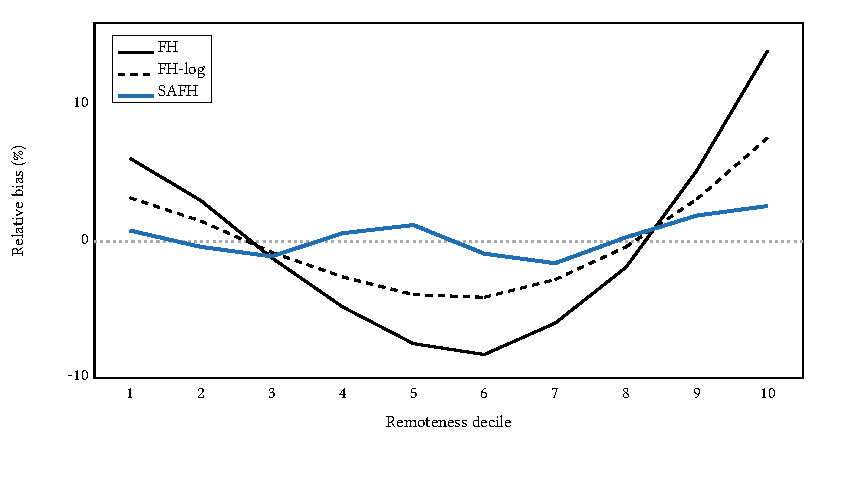
\includegraphics[width=0.85\textwidth]{figures/sim_bias.pdf}
\caption{Average relative bias of the FH, FH-log and SAFH estimators by decile
of the remoteness index, scenario 9 (concave mean function, $m = 100$, low
area-level variance).}
\label{fig:bias}
\end{figure}

The bootstrap intervals for SAFH achieved close to nominal coverage in all
scenarios, with an average coverage of 94.1\% and no scenario below 94.5\%.
Coverage was also stable across districts: Figure~\ref{fig:coverage} shows the
district-specific coverage rates for scenario 9, which lie between 93.2\% and
96.4\% with no systematic pattern in remoteness or sample size. Intervals based
on the naive MSE estimator, by contrast, had an average coverage of only 89.7\%
for $m = 50$.

\begin{figure}[t]
\centering
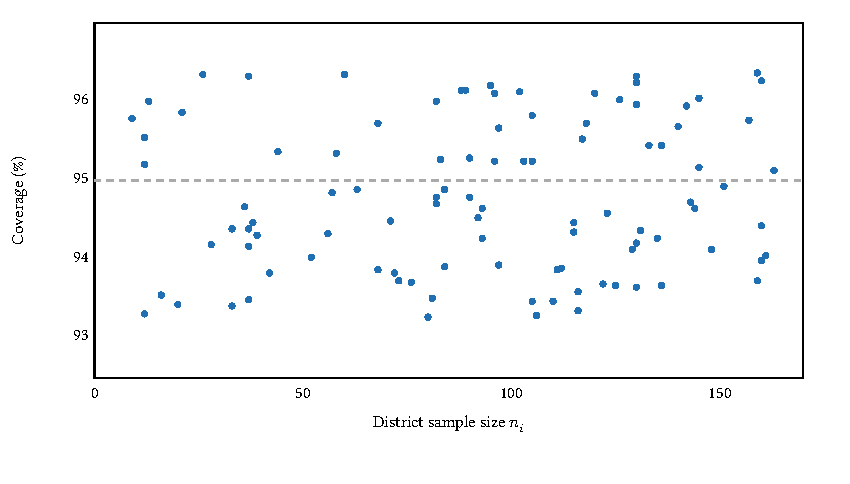
\includegraphics[width=0.85\textwidth]{figures/sim_coverage.pdf}
\caption{District-specific coverage of nominal 95\% SAFH bootstrap intervals
against district sample size, scenario 9.}
\label{fig:coverage}
\end{figure}

Table~\ref{tab:width} reports the average interval width by district sample
size. As expected, the average width of the SAFH intervals increases from
0.214 for districts with fewer than 20 sampled children to 0.081 for districts
with at least 100 sampled children, reflecting the larger weight $\hat w_i$
given to more precise direct estimates. The width of the SAFH intervals is on
average 6\% larger than that of the FH intervals, which is the price paid for
estimating the spline component, but this increase is concentrated in districts
with fewer than 20 sampled children.

\begin{table}[t]
\centering
\caption{Average width of nominal 95\% bootstrap intervals by district sample
size $n_i$, scenario 9.}
\label{tab:width}
\begin{tabular}{lrrr}
\toprule
District sample size & Districts (\%) & FH & SAFH \\
\midrule
$n_i < 20$           & 22 & 0.198 & 0.214 \\
$20 \le n_i < 50$    & 41 & 0.154 & 0.163 \\
$50 \le n_i < 100$   & 26 & 0.112 & 0.118 \\
$n_i \ge 100$        & 11 & 0.079 & 0.081 \\
\bottomrule
\end{tabular}
\end{table}

\section{Application to the Northern Provinces Household Nutrition Survey}
\label{sec:application}

\subsection{Data}
\label{sec:data}

The NPHNS was conducted between March and August 2021 by the provincial
statistical offices of the four northern provinces. It used a stratified
two-stage design in which enumeration areas were selected with probability
proportional to size within urban and rural strata of each province, and 12
households were selected systematically within each enumeration area. All
children aged 0--59 months in the selected households were eligible for
anthropometric measurement. The final sample comprised 9{,}412 children with
valid height-for-age measurements in 6{,}384 households, spread over the 214
districts of the four provinces. District sample sizes ranged from 7 to 163
children, with a median of 38.

Direct estimates of stunting prevalence were computed as H\'ajek-weighted
proportions. Because design-based variance estimates are themselves unstable in
districts with few sampled clusters, we smoothed them with a generalized
variance function, regressing the log of the estimated design effect on the log
of the district sample size and the number of sampled clusters, and setting
$\psi_i = \hat\theta_i^{\mathrm{syn}} (1 - \hat\theta_i^{\mathrm{syn}})\,
\hat d_i / n_i$, where $\hat\theta_i^{\mathrm{syn}}$ is a preliminary synthetic
estimate and $\hat d_i$ is the fitted design effect. The fitted design effects
ranged from 1.3 to 2.6.

The linear part of the model includes five district-level covariates taken from
the 2020 population census and administrative registers: the proportion of
households with an improved water source, the proportion of women aged 15--49
with completed secondary education, the proportion of households owning
livestock, the mean household size, and an indicator for districts that host a
provincial capital. The remoteness index $r_i$ was computed from a gridded
travel-time surface and district population grids; its median across districts
was 1.8 hours, with a maximum of 7.4 hours. As a secondary measure of access,
the mean distance from a household to the nearest health facility ranged from
2.1 to 38.5\,m across districts.

\subsection{Model fitting}

We fitted the FH, FH-log and SAFH models to the 214 district direct estimates.
The SAFH model used $K = 35$ knots. Table~\ref{tab:app} reports the estimated
variance components and summaries of the precision of the resulting district
estimates. Allowing a nonlinear effect of remoteness reduced the estimated
area-level variance from $\hat\sigma_u^2 = 0.0031$ under FH to
$\hat\sigma_u^2 = 0.0019$ under SAFH, indicating that a substantial part of the
between-district variation that the linear model attributes to unexplained
area effects is in fact explained by remoteness. A likelihood ratio test of
$H_0\colon \sigma_\gamma^2 = 0$, using the 50:50 mixture of $\chi^2_0$ and
$\chi^2_1$ distributions as the reference distribution
\citep{crainiceanu2004likelihood}, gave $p = 0.41$, so we reject the null
hypothesis of a linear remoteness effect.

The estimated function $\hat f$ increases steeply over the first two hours of
travel time and is nearly flat beyond four hours. Districts at a travel time of
four hours have an estimated prevalence about 9 percentage points higher than
otherwise similar districts at 30 minutes, whereas the FH model, constrained to
a straight line, implies a difference of only 5 percentage points over the same
range but overstates the difference for the few districts beyond six hours.

\begin{table}[t]
\centering
\caption{Estimated area-level variance and precision of the district estimates
under the three models, NPHNS 2021 ($m = 241$ districts). CV, coefficient of
variation.}
\label{tab:app}
\begin{tabular}{lrrr}
\toprule
 & FH & FH-log & SAFH \\
\midrule
$\hat\sigma_u^2$                    & 0.0031 & 0.0024 & 0.0019 \\
Median CV                           & 0.26   & 0.22   & 0.19   \\
Districts with CV $> 0.3$           & 61     & 38     & 23     \\
Districts with prevalence $> 25\%$  & 7      & 9      & 11     \\
\bottomrule
\end{tabular}
\end{table}

\subsection{District estimates}

The SAFH estimates are considerably more precise than the direct estimates, whose
median CV is 0.47, and also more precise than the FH estimates. The median CV of
the district estimates fell from 0.26 under FH to 0.19 under SAFH, a reduction
of 27\%, and the number of districts with a CV above 0.3, a threshold commonly
used by national statistical offices to decide whether an estimate can be
published, fell from 61 to 17. The gains are largest in the remote districts of
the two easternmost provinces, which have both the smallest samples and the
most extreme values of the remoteness index.

Figure~\ref{fig:map} maps the SAFH estimates. Under SAFH, eleven districts have
an estimated stunting prevalence above the national target of 25\%, compared
with seven under FH. All four additional districts lie in the eastern
highlands at travel times of two to four hours, where the FH model
underestimates prevalence because its linear remoteness term cannot follow the
curvature of $\hat f$. The national programme planned to prioritize districts above the target,
so the choice of model directly affects the allocation of the supplementary
feeding programme.

\begin{figure}[t]
\centering
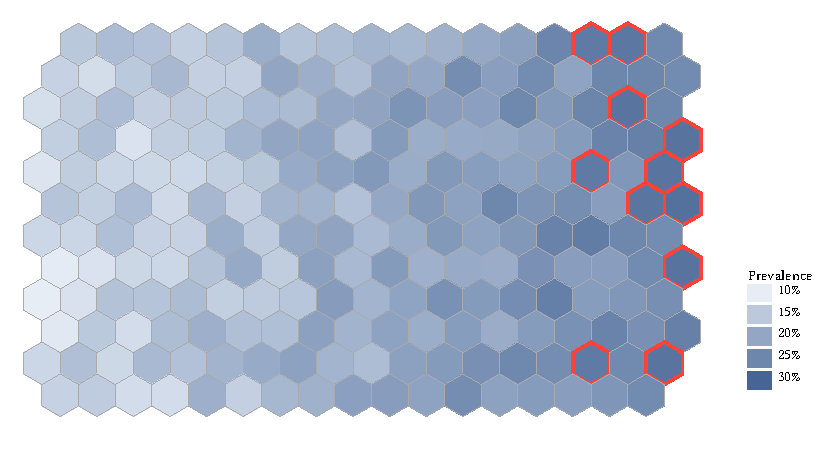
\includegraphics[width=0.8\textwidth]{figures/district_map.pdf}
\caption{SAFH estimates of stunting prevalence by district, NPHNS 2021.
Districts with an estimated prevalence above 25\% are outlined.}
\label{fig:map}
\end{figure}

As a design-based check, we compared the model-based estimates aggregated to the
provincial level with the direct provincial estimates, which are reliable at
that level. The SAFH estimates aggregated with census population weights
differed from the direct provincial estimates by at most 0.6 percentage points,
compared with up to 1.4 percentage points for FH, suggesting that the SAFH
estimates are well calibrated.

\section{Discussion}
\label{sec:discussion}

We have proposed a spline-augmented Fay--Herriot estimator that relaxes the
linearity of the regression mean for a single continuous covariate while
retaining the simplicity of an area-level model. Because the spline is
represented as a second random effect, the model can be fitted with standard
REML machinery, and the smoothing parameter is selected automatically as part
of the variance component estimation. The parametric bootstrap provides MSE
estimates that account for the estimation of both variance components, and our
simulations indicate that the resulting intervals have close to nominal
coverage even with as few as 50 districts.

In the NPHNS application, the SAFH estimator changed the substantive
conclusions in a policy-relevant way: four additional districts were classified
as exceeding the national stunting target, all of them in the eastern
highlands, where the standard model underestimates prevalence. This illustrates
a general point about small area estimation that is easy to overlook. Model
misspecification does not merely add noise to the district estimates; it
produces bias that is correlated with district characteristics, and because
shrinkage is strongest where samples are smallest, the bias is concentrated in
the districts that are usually of greatest policy interest.

Several limitations should be noted. First, the SAFH model allows a nonlinear
effect for only one covariate. Additive models with several smooth terms are a
natural extension, but with a few hundred districts the data contain limited
information about several smooth functions simultaneously, and we expect the
REML estimates of the corresponding variance components to be unstable. Second,
like all Fay--Herriot type models, SAFH treats the smoothed sampling variances
$\psi_i$ as known. Errors in the generalized variance function propagate to the
weights $\hat w_i$, and a fully Bayesian treatment that models the sampling
variances jointly with the prevalences would be a useful extension
\citep{you2006small}. Third, the remoteness index is itself estimated from a
travel-time surface, and measurement error in $r_i$ could attenuate the
estimated function $\hat f$ \citep{ybarra2008small}.

Several limitations should be noted. First, the SAFH model allows a nonlinear
effect for only one covariate. Additive models with several smooth terms are a
natural extension, but with a few hundred districts the data contain limited
information about several smooth functions simultaneously, and we expect the
REML estimates of the corresponding variance components to be unstable. Second,
like all Fay--Herriot type models, SAFH treats the smoothed sampling variances
$\psi_i$ as known. Errors in the generalized variance function propagate to the
weights $\hat w_i$, and a fully Bayesian treatment that models the sampling
variances jointly with the prevalences would be a useful extension
\citep{you2006small}. Third, the remoteness index is itself estimated from a
travel-time surface, and measurement error in $r_i$ could attenuate the
estimated function $\hat f$ \citep{ybarra2008small}.

Finally, the estimated function $\hat f$ should not be given a casual
interpretation. Remoteness is correlated with many unobserved determinants of
child growth, including dietary diversity, disease burden and access to
antenatal care, and the SAFH model is designed for prediction rather than for
identifying the effect of travel time on stunting. Policies that reduce travel
times, such as road construction, may therefore have effects on nutrition that
differ substantially from what the slope of $\hat f$ would suggest.

The approach extends directly to other indicators routinely published from
household surveys, such as wasting, underweight or vaccination coverage, and to
other auxiliary variables with a plausibly nonlinear relationship to the
outcome, such as night-time light intensity or population density. An
implementation in R is provided in the supplementary material.


\section*{Acknowledgements}
We thank the field teams of the Northern Provinces Household Nutrition Survey
and the provincial statistical offices for access to the survey microdata and
district boundary files. The work was supported by a research grant from the
Lowmoor Centre for Health Data Science.

\section*{Data availability}
District-level direct estimates, design-based variances and covariates used in
Section~\ref{sec:application} are available from the corresponding author on
reasonable request. Code implementing the SAFH estimator is provided as
supplementary material.

\bibliographystyle{plainnat}
\bibliography{refs}

\appendix
\section{Parametric bootstrap for the MSE}
\label{app:bootstrap}

Let $\hat\bbeta^{*}$, $\hat\sigma_u^2$ and $\hat\sigma_\gamma^2$ denote the REML
estimates obtained from the observed data. For $b = 1, \dots, B$ we proceed as
follows.
\begin{enumerate}
  \item Generate $\gamma_k^{*(b)} \sim N(0, \hat\sigma_\gamma^2)$ for
  $k = 1, \dots, K$, $u_i^{*(b)} \sim N(0, \hat\sigma_u^2)$ and
  $e_i^{*(b)} \sim N(0, \psi_i)$ for $i = 1, \dots, m$, all independently.
  \item Compute the bootstrap true values
  $\theta_i^{*(b)} = \bx_i^\top \hat\bbeta + \hat\beta_r r_i +
  \boldsymbol{z}_i^\top \boldsymbol{\gamma}^{*(b)} + u_i^{*(b)}$ and the
  bootstrap data $y_i^{*(b)} = \theta_i^{*(b)} + e_i^{*(b)}$.
  \item Re-estimate the model from $\{y_i^{*(b)}, \bx_i, r_i, \psi_i\}$ by REML
  and compute the bootstrap predictor $\hat\theta_i^{*(b)}$.
\end{enumerate}
The bootstrap MSE estimator \eqref{eq:boot-mse} estimates the MSE of the
predictor including the variability due to the estimation of
$\boldsymbol{\delta}$. Following \citet{butar2003measuring}, we use the
bias-corrected estimator
\begin{equation}
  \mathrm{mse}_{BC}(\hat\theta_i^{\mathrm{SAFH}}) =
  2\, g_{1i}(\hat{\boldsymbol{\delta}}) - \frac{1}{B} \sum_{b=1}^{B}
  g_{1i}(\hat{\boldsymbol{\delta}}^{*(b)})
  + \frac{1}{B} \sum_{b=1}^{B}
  \left( \hat\theta_i^{*(b)} - \tilde\theta_i^{*(b)} \right)^2,
  \label{eq:boot-bc}
\end{equation}
where $g_{1i}(\boldsymbol{\delta}) = w_i \psi_i$ is the leading term of the MSE
of the best predictor and $\tilde\theta_i^{*(b)}$ is the best predictor computed
with the true bootstrap parameters. If \eqref{eq:boot-bc} is negative, which
happened in fewer than 0.1\% of district-replicate combinations in our
simulations, we replace it by $g_{1i}(\hat{\boldsymbol{\delta}})$.

Each bootstrap replicate requires one REML fit. With $m = 214$ and $K = 35$,
a single fit takes about 40 milliseconds on a standard laptop, so that
$B = 1000$ replicates take well under a minute.


\end{document}
